\begin{frame}{Introduction}
		HgTe is a II-VI semiconductor and a topological insulator (TI).\footfullcite{top_surf_states}
		\vspace{10px}
	\begin{columns} 
		\begin{column}<2->{0.35\linewidth} \centering
			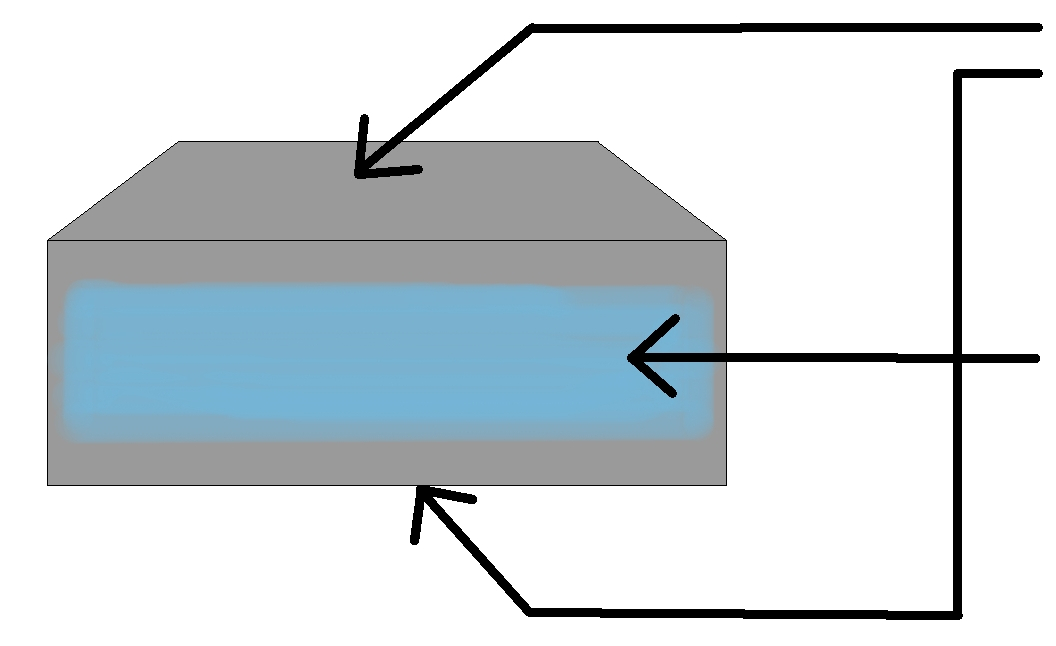
\includegraphics[width=\linewidth]{extrabilder_fuer_vortrag/Introduction1.jpg}
		\end{column}
		\begin{column}<2->{0.23\linewidth} 
			conducting surface states
			
			\vspace{5px}
			insulating in the bulk
			
			\vspace{15pt}
		\end{column}\hfill
		\begin{column}<3->{0.5\linewidth} 
			TIs are interesting because:
			\begin{itemize}
				\item<4-> spin-momentum locking
				\item<5-> protected surface states
			\end{itemize}
		\end{column}\hfill
	\end{columns}
	
	\note{HgTe belongs to the class of mercury-based II-VI semiconductors which appear in zinc-blende structure. It is additionally found to be a topological insulator.\\
	A topological insulator is a material which is insulating in its interior, also called the bulk of a material, and that develops conducting states at the surface.\\
	They are very attractive for potential applications because the spin and the momentum of the electrons at the conducting surfaces are locked. This means, the spin is always perpendicular to the direction of motion of those electrons.
	The spin-momentum locking make sure that the surfaces are protected if time-reversal symmetry preserved. In other words the surface states remain even for non-magnetic impurities.\\}
	\begin{columns}
		\begin{column}<6->{\linewidth}
		Calculations were performed using density functional theory (DFT) through FHI-aims.
		\end{column}
	\end{columns}	
	\begin{columns}<7->
		\begin{column}{0.1\linewidth}
			\vspace{9px}
			$0.5 \unit{nm}~\approx$
		\end{column}
		\begin{column}{0.8\linewidth}
			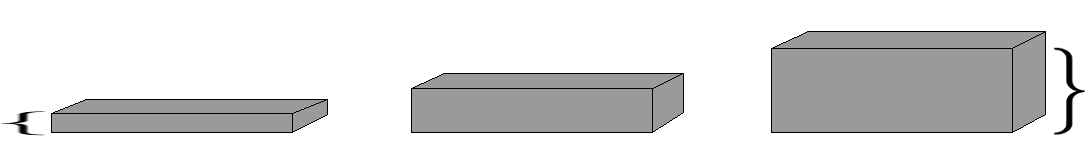
\includegraphics[width=\linewidth]{extrabilder_fuer_vortrag/Introduction2.jpg}
		\end{column}
			\hspace{-15px} 
		\begin{column}{0.1\linewidth}
			\vspace{.2px}
			$\approx~2.7 \unit{nm}$
		\end{column}
	\end{columns}
	\note{The calculations I performed were ab-initio calculations and therefore I used the density functional theory with the exchange-correlation function method PBE, which is short for Perdew-Burke-Ernzerhof through FHI-aims.\\}
	\note{HgTe was examined in thin films from approximately 0.5 nm to 2.7 nm, which are 4 to 17 layers of atoms. Surfaces can only be examined in one direction at once. Because otherwise it would went beyond the scope of a bachelor thesis, we chose just direction of observance, namely the (001) direction. \\
	The main goal this thesis pursued was examining the evolution of topological surface states for different slab thicknesses. Therefore I will now explain the theory behind the realization of this examination.}
	\begin{block}<8->{}
		Main goal: Evolution of surface states in different slab thicknesses.
	\end{block}
\end{frame}

%%% Local Variables:4
%%% mode: latex
%%% TeX-master: "main_BA2_Vortrag.tex"
%%% End: